%!TEX root = main.tex
\documentclass[main.tex]{subfiles}

\begin{document}


% As introduced in the first chapter, the transcription of target languages in language documentation workflows can be incredibly time-consuming, taking 30--50 hours of work to transcribe an hour of recorded speech.~Automatic speech recognition (ASR) could potentially speed up this process by helping obtain human-correctable first-pass transcriptions.~However, ASR systems are typically unavailable for many minoritised languages as their development has conventionally required at least tens if not several hundreds of hours of transcribed speech --- leaving many minoritised languages in a Catch-22.~The recent emergence of large-scale pre-trained models may provide a path forward, given their advertised ability to learn new tasks with little task-specific data.~In this chapter and the next, I examine whether we can leverage these models with only limited amounts of transcriptions along with supplemental resources to obtain ASR systems capable of delivering human-correctable first-pass transcriptions.~In this chapter, I examine whether 10 minutes of transcriptions may be sufficient to obtain such a system if some text data is also available. 

\vspace{2em}

\chapter{Leveraging untranscribed speech to adapt pre-trained models for under-represented languages}
\chaptermark{Leveraging untranscribed speech for model adaptation}

\vspace{2em}

As in the previous chapter, I continue to examine how to effectively use limited target language transcriptions by leveraging other resources.~As introduced previously, the ability to train models using only untranscribed speech through `pre-training' has enabled speech processing models to leverage hundreds of thousands of hours of data.~Yet, as the available large-scale speech datasets are dominated by major European languages, these pre-trained models are not well-adapted for languages under-represented in these datasets, resulting in relatively poorer performance when subsequently trained or `fine-tuned' for ASR on an under-represented target language.~To adapt the pre-trained model for a target language using only untranscribed recordings, I examine the method of `continued pre-training', which, as its name suggests, involves continuing to train the model in the same manner, but using untranscribed speech from the target language.~However, since these models are designed to be trained using considerable quantities of data, continuing to train them using only a comparatively small amount of untranscribed speech may reduce the effectiveness of the process.~In this chapter, I examine whether the effectiveness of continued pre-training can be maximised by also drawing upon untranscribed speech from a similar language for which larger quantities are available and also explore how best to select this similar language (henceforth the `donor' language).

\section{Background}
\label{sec:sigtyp:bg}

For developing automatic speech recognition (ASR), `low resource' languages are typically classified as such based on the availability of transcribed speech.~Untranscribed speech or reliable metadata about the language are often assumed to be easily obtainable.~This assumption may not hold true for under-described languages with little digital representation.~For such languages, I address two questions in this chapter:~1) does leveraging untranscribed speech from a similar, higher-resource `donor' language for pre-trained model adaptation help improve speech recognition in the target language,~and 2) how do we select the best donor?

The first question is of interest as ASR system development with little transcribed speech has become viable with multilingual pre-trained transformer models for speech ~\parencite[e.g.~wav2vec 2.0 XLSR-128:][]{babu22_interspeech}.~Yet, as most languages are under-represented in the pre-training data, directly fine-tuning these models with transcribed speech for ASR in the target language can yield lower performance compared to their well-represented counterparts \parencite{conneau2023fleurs}.~While recent studies have shown the effectiveness of continued pre-training to adapt these models using untranscribed speech from the target language~\parencite{NOWAKOWSKI2023103148,paraskevopoulos2024sample}, they involved using 70--200 hours of target language data.~For some languages, it may be quite difficult to source this much speech data --- even untranscribed.

The second question is of interest as under-described languages face a similar issue of under- and even \emph{mis-}representation in typological databases such as lang2vec \parencite{littell2017uriel}, which itself draws on other databases \parencite[e.g.~phonological information from WALS:][]{haspelmath2009typological}.~For example, as phonological information for Punjabi is not available in WALS, the feature vector within lang2vec is derived by averaging information from neighbouring languages, and this leads to erroneous similarity scores when such data is used for comparisons.~Thus, it is unclear whether existing similarity measures can robustly help select a suitable donor language and, further, to what extent these measures are suitable for predicting ASR performance differences as a result of continued pre-training.

Addressing these two questions, this chapter proceeds as follows.~In the remainder of this section (§\ref{sec:sigtyp:bg}), I provide an overview of the continued pre-training (CPT) task and highlight certain details about the wav2vec 2.0 architecture that will be relevant to later discussions for developing a suitable, predictive measure.~Subsequently (§\ref{sec:sigtyp:exp1}), I present the results of CPT experiments using Punjabi as a target language and sourcing donor data from 8 other Indic languages.~In the following section (§\ref{sec:sigtyp:atds}), I motivate, analyse, and validate the Acoustic Token Distribution Similarity (ATDS) --- a bottom-up acoustic measure for language similarity between a target and donor.~Validation experiments on Punjabi as well as three additional languages (Galician, Iban, Setswana) show that the ATDS precisely predicts target language ASR performance as a result of CPT-based adaption using a mix of target and donor data and outperforms all other measures examined.~Finally (§\ref{sec:sigtyp:conc}), I summarise the findings of this chapter, making clear their limitations and outlining directions for future research.

\subsection{Continued pre-training: model adaptation using untranscribed speech}

As introduced in the second chapter (§\ref{sec:chp2-FMs}), pre-training involves the use of a proxy task which is able to leverage unlabelled data (e.g.~untranscribed speech).~This allows for models such as wav2vec 2.0 XLSR-128 to be pre-trained at very large scales, e.g.~using 436k hours of untranscribed speech as illustrated by Stage 1a in Figure \ref{fig:sigtyp2021-cpt}.~However, many languages are under-represented in the standard datasets used for this initial pre-training.~As such, directly fine-tuning these models for under-represented target languages (i.e.~direct from Stage 1a to 2 for Punjabi in Figure \ref{fig:sigtyp2021-cpt}) results in relatively reduced ASR performance compared to their well-represented, European counterparts.
\newpage

\begin{figure}[ht]
  \centering
  % \vspace{1em}
  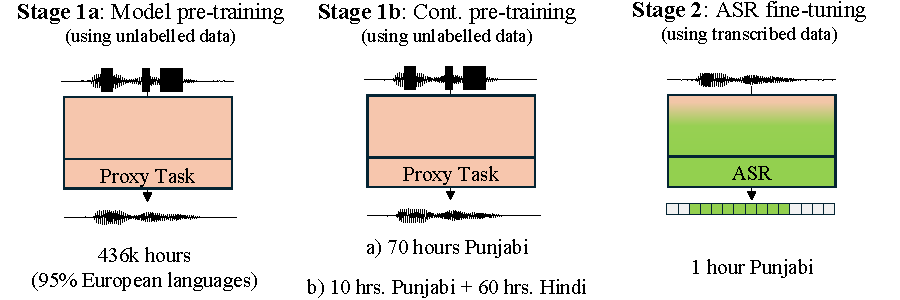
\includegraphics[width=0.8\linewidth]{figures/sigtyp2024-cpt-paradigm}
  % \vspace{-1em}
  \caption[Model adaptation via continued pre-training]{Continued pre-training using untranscribed speech from a) large amounts of speech from only the target language (e.g.~70 hours of Punjabi) or b) a mix of the target and a similar, higher-resource `donor' language (e.g.~10 hours of Punjabi and 60 hours of Hindi).}
  \label{fig:sigtyp2021-cpt}
\end{figure}

Given that recording speech is much simpler than transcribing speech, there typically exists far more untranscribed speech than transcribed.~Making use of this fact, recent studies \parencite[e.g.][]{NOWAKOWSKI2023103148,paraskevopoulos2024sample} have shown that these models can be adapted for the target language simply by additional or `continued' pre-training (CPT) using the larger amounts of untranscribed speech, e.g.~using 70 hours of Punjabi in Figure \ref{fig:sigtyp2021-cpt} a).~However, such large amounts of speech data may not exist for many digitally under-represented languages.~For these languages, we are interested in whether CPT-based adaptation can yield similar levels of improvements when supplementing target language data with data from similar, higher-resource `donor' language, e.g.~using 10 hours of Punjabi with 60 hours of Hindi in Figure \ref{fig:sigtyp2021-cpt} b).

\subsection{wav2vec 2.0}

As introduced in the second chapter (§\ref{sec:chp2-w2v2}), wav2vec 2.0 is a pre-trained model developed for speech processing.~We highlight here two important details relevant for our later discussions.~The first is that the representations learned by the transformer network are particularly useful for speech applications requiring fine-grained comparisons of acoustic-phonetic content,~e.g.~speech information retrieval \parencite{san2021leveraging}, second language pronunciation scoring \parencite{bartelds2022neural,richter2023relative}, spoken dialect classification \parencite{bartelds-wieling-2022-quantifying,guillaume23_sigul} --- particularly those learned by the middle layers of the transformer network (e.g.~layers 12--16 of a 24-layer network).

\begin{figure}[!ht]
    \vspace{-0.5em}
    \centering
    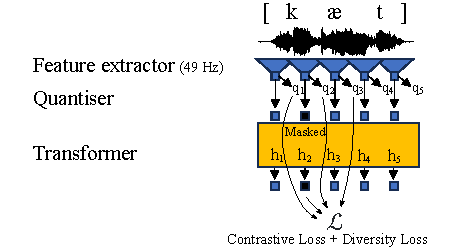
\includegraphics[width=0.5\linewidth]{figures/sigtyp2024-w2v2-v2}\vspace{-0.5em}
    \caption[Illustration of the wav2vec 2.0 architecture]{Illustration of the wav2vec 2.0 architecture. Adapted from \textcite{NEURIPS2020_92d1e1eb}.}
    \label{fig:w2v2}
\end{figure}

The second detail is that these representations are encoded as vectors in a high-dimensional latent space and emitted at a rate of 49 Hz.~Combined with the diversity loss that requires exploration of this space, there is a many-to-many relationship between phonetic categories and these vectors --- both in the latent space and in time.~For example, as illustrated in Figure \ref{fig:w2v2}, a single speech sound such as [\ae] may last for three time steps (yielding $h_2, h_3, h_4$).~The first two vectors ($h_2, h_3$) may be very close in the latent space, as they map to the start of [\ae] sounds while the third $h_4$ may map to [\ae] sounds preceding [t] and is thus located in a different part of the latent space.~Thus to derive phone-like tokens from these representations, we must group them in the latent space (e.g.~using \textit{k}-means clustering) and then again in time according to how the grouped units themselves routinely co-occur (e.g.~using subword modelling).

~In this way, the goal of tokenisation for both text and speech is driven by the need to derive units of a practical granularity based on the nature of the input: from coarser-grained words to finer-grained sub-words in text and, inversely, finer-grained sub-phones to coarser-grained phones in speech.~We return to these two details in our development of the Acoustic Token Distribution Similarity measure for comparing the acoustic-phonetic similarity of two untranscribed speech corpora.

\section{Experiment 1: A systematic study of pairwise transfer}
\label{sec:sigtyp:exp1}

% \subsection{Motivation}
% \label{sub_sec:pair_motivation}

% Since the release of the original English wav2vec 2.0 model pre-trained on the 960 hour LibriSpeech corpus~\parencite{7178964}, additional massively multi-lingual variants have also been developed: XLSR-53, pre-trained on 56k hours from 53 languages~\parencite{conneau21_interspeech}; XLSR-128, pre-trained on 436k hours from 128 languages~\parencite{babu22_interspeech}; and MMS, pre-trained on 491k hours from 1,406 languages \parencite{pratap2023scaling}.~In each case, the vast majority of the pre-training data is drawn from European language sources.

Given the under-represented nature of most languages in these wav2vec 2.0 models, several studies have investigated continued pre-training (CPT) to adapt them for target languages \parencite[e.g.][]{javed2021building,dehaven2022improving,NOWAKOWSKI2023103148,bartelds-etal-2023-making,paraskevopoulos2024sample}.~\textcite{NOWAKOWSKI2023103148} adapted the XLSR-53 model using 200 hours of Ainu.~Using the same 40 minutes of transcribed Ainu for ASR fine-tuning,~they found that the adapted model resulted in a 8.8\% absolute word error rate (WER) decrease over the off-the-shelf XLSR-53 model.~For many low resource languages, however, obtaining 200 hours of speech data may not be feasible.~In their study of unsupervised domain adaptation for Greek,~\textcite{paraskevopoulos2024sample} found adapting the XLSR-53 model via CPT using a small 12-hour dataset of Greek read speech to be ineffective.~However, they found that successful CPT-based adaptation could be achieved with the use of multi-domain data,~e.g.~12 hours of read speech mixed with 70 hours of newscasts.~Given these findings, we were motivated to investigate whether comparable results could be achieved by supplementing target language data with data from another.

\subsection{Method}

\textbf{\textit{Model training}}.~As our primary interest was in examining how downstream ASR performance is affected by the dataset(s) used in continued pre-training (CPT), we carried out nearly identical experiments as those in \textcite{NOWAKOWSKI2023103148} by obtaining their configuration file for wav2vec 2.0 pre-training.~Similarly, we follow the official ASR fine-tuning recipe suitable for 1 hour of transcriptions.~For both procedures, we made modifications to suit our hardware configuration and compute budget, as detailed in Appendix \ref{sec:appendix-sigtyp2024}.

\noindent{}\textbf{\textit{Data}}.~For a systematic investigation of how downstream ASR performance in a given target language varies with the choice of supplemental language added during CPT, we required a dataset with some specific characteristics: a) contains a variety of both similar and dissimilar languages with, b) at least 60 hours per language, c) and collected in relatively similar acoustic conditions, and d) not have already been used in the original pre-training process.~Accordingly, for this set of experiments, we sourced data from IndicSUPERB \parencite{10.1609/aaai.v37i11.26521}, a dataset of 12 Indic languages containing 65--180 hours of read speech per language.

Amongst these 12 IndicSUPERB languages, we selected Punjabi as our target language as it is relatively low-resourced (cf.~Hindi, Tamil), its geographical and typological location (yielding a variety of closer and farther geographic/typological distances to the others), and also native speaker-linguist expertise on our research team for data validation and error analysis.

As illustrated in Figure \ref{fig:indic_data}, we began by selecting for our top-line condition a random 70h subset of Punjabi from the total 136h available in IndicSUPERB, and then from this subset a random 10h selection for our baseline, and again a random 1h subset for fine-tuning.~We also selected a random 1h validation and 2h test set both disjoint from each other and any data to be used for pre-training.

\begin{figure}[H]
    \centering
    % \vspace{-0.5em}
    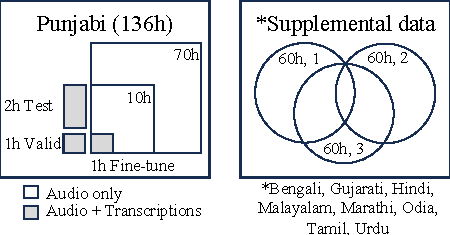
\includegraphics[width=0.45\linewidth]{figures/sigtyp2024-indicsuperb}
    \vspace{-1em}
    % \vspace{-0.5em}
    \caption{Data selection for transfer experiments}
    \label{fig:indic_data}
    \vspace{-1em}
\end{figure}

Additionally, for each donor language (Bengali, Gujarati, Hindi, Malayalam, Marathi, Odia, Tamil, Urdu), we created three random 60h subsets.~Given the total amounts of data available in IndicSUPERB for each language (e.g.~87h for Urdu but 129h for Gujarati), there is however some unavoidable overlap between these subsets for each language (i.e.~they are not disjoint 60h splits).~Using each of the 60h subsets, we conducted 3 separate CPT runs per language to obtain estimates for both within- and between-donor language differences on downstream ASR performance.

\subsection{Results and discussion}

\begin{figure}[!b]
\definecolor{mygray}{gray}{0.9}
\centering
\scalebox{0.85}{
\renewcommand{\arraystretch}{1}
\begin{tabular}{@{}llcl@{}}
\toprule
\multirow{1}{*}{\makecell{\vspace{-0.45em}\\Condition}}     & \multicolumn{2}{c}{Test set WER (WERR)}                                                & \multirow{1}{*}{\makecell{\vspace{-0.45em}\\Data for continued pre-training}}          \\ \cmidrule(r){2-3}  
                               & \multicolumn{1}{c}{Median}         & \multicolumn{1}{c}{Range}                     &                         \\ \midrule

T.\hspace{0.87em}In-domain top-line         & 22.2 (11.2\%)  & -                                                                      & 70h Punjabi                                    \\  \cmidrule{1-4} 
E1. Most similar   & \textbf{23.5 (6.0\%)}     & 23.4--23.8   & 10h Punjabi + 60h Hindi                          \\ \cmidrule{1-4}
\multirow{3}{*}{\makecell{\vspace{-0.45em}\\E2. Similar}}   & 24.4 (2.4\%)   & 24.3--24.5     & 10h Punjabi + 60h Urdu                            \\ \cmidrule{2-4}
   & 24.4 (2.4\%)   & 24.2--24.4   & 10h Punjabi + 60h Gujarati                       \\  \cmidrule{2-4}
   & 24.6 (1.6\%)   & 24.5--24.7 & 10h Punjabi + 60h Marathi                         \\  \cmidrule{1-4}

\rowcolor{mygray} B.\hspace{0.75em}Only target data baseline & 25.0     & -                                                                      & 10h Punjabi                                      \\  \cmidrule{1-4} 
\multirow{4}{*}{\makecell{\vspace{-0.1em}\\E3. Unrelated/dissimilar}} & 25.0 (0.0\%)     & 25.0--25.2    & 10h Punjabi + 60h Odia                             \\  \cmidrule{2-4} 
         & 25.1 (-0.4\%)  & 25.0--25.4    & 10h Punjabi + 60h Tamil                            \\ \cmidrule{2-4}
         & 25.1 (-0.4\%)  & 25.0--25.3    & 10h Punjabi + 60h Malayalam                        \\  \cmidrule{2-4}
& 25.2 (-0.8\%)  & 25.1--25.2  & 10h Punjabi + 60h Bengali    \\ 
 \cmidrule{1-4}
U.\hspace{0.75em}Unadapted XLSR-128     & 30.8 (-23.2\%) &  -                                                                     & -                                               \\ \bottomrule
\end{tabular}
% \vspace{-2em}
}

\captionof{table}[Automatic speech recognition results from fine-tuning wav2vec 2.0 models with and without adaptation via continued pre-training]{Automatic speech recognition (ASR) results from fine-tuning wav2vec 2.0 XLSR-128 \cite{babu22_interspeech} with and without adaptation via continued pre-training (CPT). CPT-adapted models were trained for 10k updates using 70 hours of Punjabi for the topline (T), 10 hours of Punjabi for the baseline (B), and 10 hours of Punjabi combined with 60 hours of data from another language for the experiment conditions (E1, E2, E3).~All models were fine-tuned with the same 1 hour of Punjabi data.~ASR performance reported in word error rate (WER; lower is better) and word error rate reduction (WERR; higher is better) relative to the 10 hour CPT baseline (B).~For each experiment condition, median and range were obtained from 3 CPT runs per language with different donor data in each run.}
% For each language in the experiment conditions, three separate CPT runs each using different 60h subsets of the language were conducted (yielding a min, median, and max WER). 
\label{tab:indic_results}


\end{figure}


Compared to directly fine-tuning the XLSR-128 model, adapting the model first via continued pre-training (CPT) with 70 hours of Punjabi yields a large improvement in downstream ASR performance (unadapted 30.8\%~vs.~22.2\% CPT-adapted, 70h).~This constitutes an absolute WER difference of 8.6\% and is consistent with improvements reported in previous CPT experiments \cite[][]{NOWAKOWSKI2023103148,paraskevopoulos2024sample}.~We found that model adaptation with only 10 hours of Punjabi still yielded an appreciable improvement over the unadapted model:~5.8\% absolute (unadapted 30.8\%~vs.~25.0\% CPT-adapted, 10h).

We now turn to our experiment conditions in which 10h of Punjabi is supplemented with 60h of data from another language.~As summarised in Table \ref{tab:indic_results}, the effects of supplemental language on Punjabi ASR performance can be divided into roughly three strata.~In the bottom stratum (E3), we find unrelated Dravidian languages (Tamil, Malayalam) or dissimilar Indo-Aryan languages (Bengali, Odia).~When these languages are added as supplemental data during CPT, we find no meaningful difference compared to using only 10 hours of Punjabi (word error rate reduction, WERR: -0.8--0.0\%; n.b. higher WERR is better).

In the middle stratum (E2), we find relatively similar Indo-Aryan languages (Marathi, Gujarati, Urdu). When these languages are added as supplemental data, we find modest improvements over using only 10 hours of Punjabi (WERR: 1.6--2.4\%).~In the top stratum (E1), we find Hindi --- the most similar Indo-Aryan language amongst our candidate donors.~When Hindi is added as supplemental data, we find a large improvement over using only 10 hours of Punjabi (WERR: 6.0\%).~In fact, adding the 60h of Hindi results in ASR performance that is in absolute terms close to the 70h Punjabi topline, respectively:~23.5\% vs.~22.2\% (WER, lower is better).

We have established that there are observable differences in target language ASR performance that vary with the donor language added during continued pre-training and that these differences appear to align with qualitative notions of language similarity.~In the next section, we investigate quantitative measures of similarity and evaluate their correlations to these observed differences.

\section{Experiment 2: Evaluating predictiveness of similarity measures}
\label{sec:sigtyp:atds}

% \subsection{Motivation}

A common method for calculating similarities between languages is to use language vectors from the lang2vec database \parencite{littell2017uriel}, which itself draws on other databases \parencite[e.g.~phonological information from WALS:][]{haspelmath2009typological}.~\textcite{9688276} investigated how well measures based on lang2vec and other data sources correlated with successful transfer learning for ASR.~Of the lang2vec similarity metrics, they found that genetic and geographic measures correlated highly with better ASR performance but, surprisingly, inventory and phonological measures did not.~Acoustic similarities as derived from embeddings of a pre-trained spoken language identification model were also found to correlate strongly with better ASR performance.~In the context of continued pre-training, we questioned whether the to-be-adapted model could be used for this purpose.

Investigating an analogous question in the text domain, \textcite{gogoulou2023study} evaluated various measures for predicting transfer characteristics for transformer language models initially pre-trained on one language (e.g.~English) and subsequently adapted to another (e.g.~Icelandic), and how these characteristics varied according to the distributions of data in the respective language corpora.~They propose a novel metric:~the Token Distribution Similarity (TDS), which correlated with positive transfer.~As illustrated in Figure \ref{fig:atds} (a), the TDS is derived by 1) using the pre-trained model's tokeniser to process a sample of data from each language, 2) then generating a token frequency vector for each language, and 3) taking the cosine similarity between these two vectors.~Given these promising results for predicting positive cross-lingual transfer for continued pre-training on text, an analogous measure for speech could offer the same predictive property.

\begin{figure}[t]
\centering
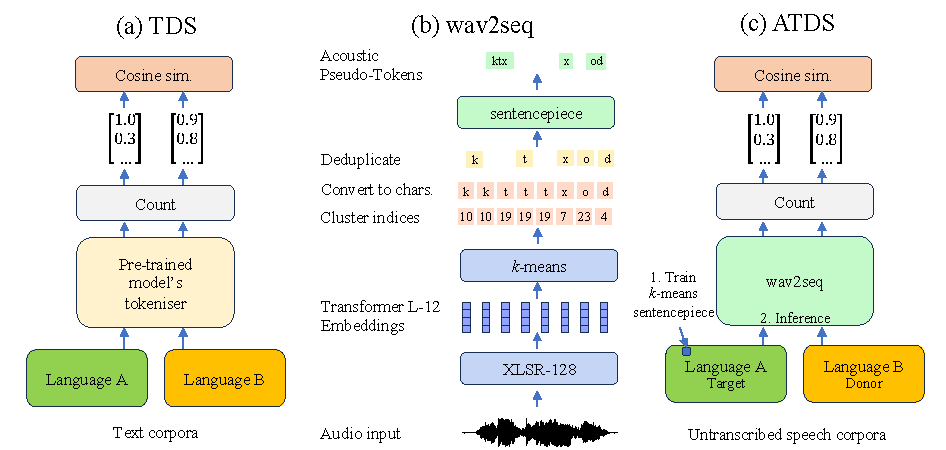
\includegraphics[width=1\textwidth]{figures/sigtyp2024-atds2.pdf}
% \caption{Derivation of the Acoustic Token Distribution Similarity (ATDS) based on adapting the Token Distribution Similarity \parencite[TDS:][]{gogoulou2023study} for untranscribed speech corpora using acoustic pseudo-tokens induced via the wav2seq method \parencite{10096988}.}
\caption[Derivation of the Acoustic Token Distribution Similarity (ATDS) measure]{\corr{Derivation of the Acoustic Token Distribution Similarity (ATDS) measure for predicting positive transfer between two languages resulting from continued pre-training (CPT) of a pre-trained speech model (e.g. XLSR-128).~ATDS extends to the speech domain the concept of Token Distribution Similarity \parencite[TDS:][]{gogoulou2023study}, shown to predict positive transfer for CPT in the text domain.~To account for the token-less nature of untranscribed speech, pseudo-tokens are derived using the wav2seq process proposed by \textcite{10096988}.~As is the case for text tokenisation, the goal is to derive units of practical granularity based on the raw input.~While typical text tokenisation sub-divides words into sub-words (e.g.~\emph{eating} $\rightarrow$ \emph{eat,ing}), the analogous process for raw speech data involves grouping sub-frames into more phone-like units: first based on featural similarity (e.g.~using a clustering method such as k-means) then again based on distributional similarity (e.g.~using sub-word modelling via the sentencepiece package).}}

\label{fig:atds}

\end{figure}

In order to compute token distribution similarity for two untranscribed speech corpora, we first need to `tokenise' the corpora.~For this purpose, it may be possible to leverage the speech representations extracted using a middle transformer layer (e.g. Layer 12 of 24) of a pre-trained wav2vec 2.0 model such as XLSR-128.~As previously highlighted above, these representations are useful for fine-grained comparisons of acoustic-phonetic content and, to make use for these representations for inducing phone-like tokens, they must first be grouped in the high-dimensional latent space and then again in time based on their co-occurrences.

Indeed, wav2seq proposes this very way of inducing pseudo-tokens.\footnote{Originally developed for inducing pseudo-tokens for use in a self-supervised pseudo speech recognition task for jointly pre-training a speech encoder and text decoder.}~As illustrated in Figure \ref{fig:atds} (b), the first step is using a pre-trained model (e.g.~XLSR-128) to extract speech embeddings from a transformer layer.~The second step involves training a \textit{k}-means model to cluster these embeddings (i.e.~group similar sounds together).~The cluster indices are converted to characters (by a simple Unicode table lookup,~e.g.10$ \rightarrow $\textit{k}, 19$\rightarrow$\textit{t}, etc.)~and then deduplicated.~To discover frequently occurring sound sequences, the third step involves using these character strings to train a subword model \parencite[e.g.~via sentencepiece:][]{kudo2018sentencepiece}.~Once these models are trained on a subset of the corpus, they are used to derive pseudo-tokens for the rest of the corpus and, in our application, also for candidate donor corpora.

Accordingly, we propose the \textit{Acoustic} Token Distribution Similarity (ATDS) measure, which, as illustrated in Figure \ref{fig:atds} (c), is a straightforward composition of wav2seq \parencite{10096988} and Token Distribution Similarity \parencite[TDS:][]{gogoulou2023study}.~In the remainder of this section, we provide 1) a sanity check of the induced pseudo-tokens and 2) two analyses showing that the ATDS between a target language and its candidate donors precisely predicts downstream ASR performance in the target language resulting from continued pre-training of a speech model on target and donor data.

\subsection{Sanity check of acoustic pseudo-tokens}

\corr{{\textbf{\textit{Method}}. To discover whether these pseudo-tokens exhibited both within- and cross-language consistency, we conducted an analysis using the Punjabi and Hindi datasets of the CommonVoice corpus \parencite{ardila2019common}, for which forced-aligned phoneme labels are available as TextGrids in the VoxCommunis corpus \parencite{ahn-chodroff-2022-voxcommunis}.~For this analysis, we trained the \textit{k}-means and subword models on Punjabi (the target language) and then induced pseudo-tokens for both Punjabi and Hindi.~We then appended additional tiers containing the time intervals for these pseudo-tokens to TextGrids containing phoneme labels sourced from VoxCommunis and analysed their correspondences.~Figure \ref{fig:textgrid} illustrates a span of a Punjabi utterance enriched with \unskip\parfillskip 0pt \par}}

\begin{landscape}

\begin{figure}[t]
\centering
\vspace{-2em}
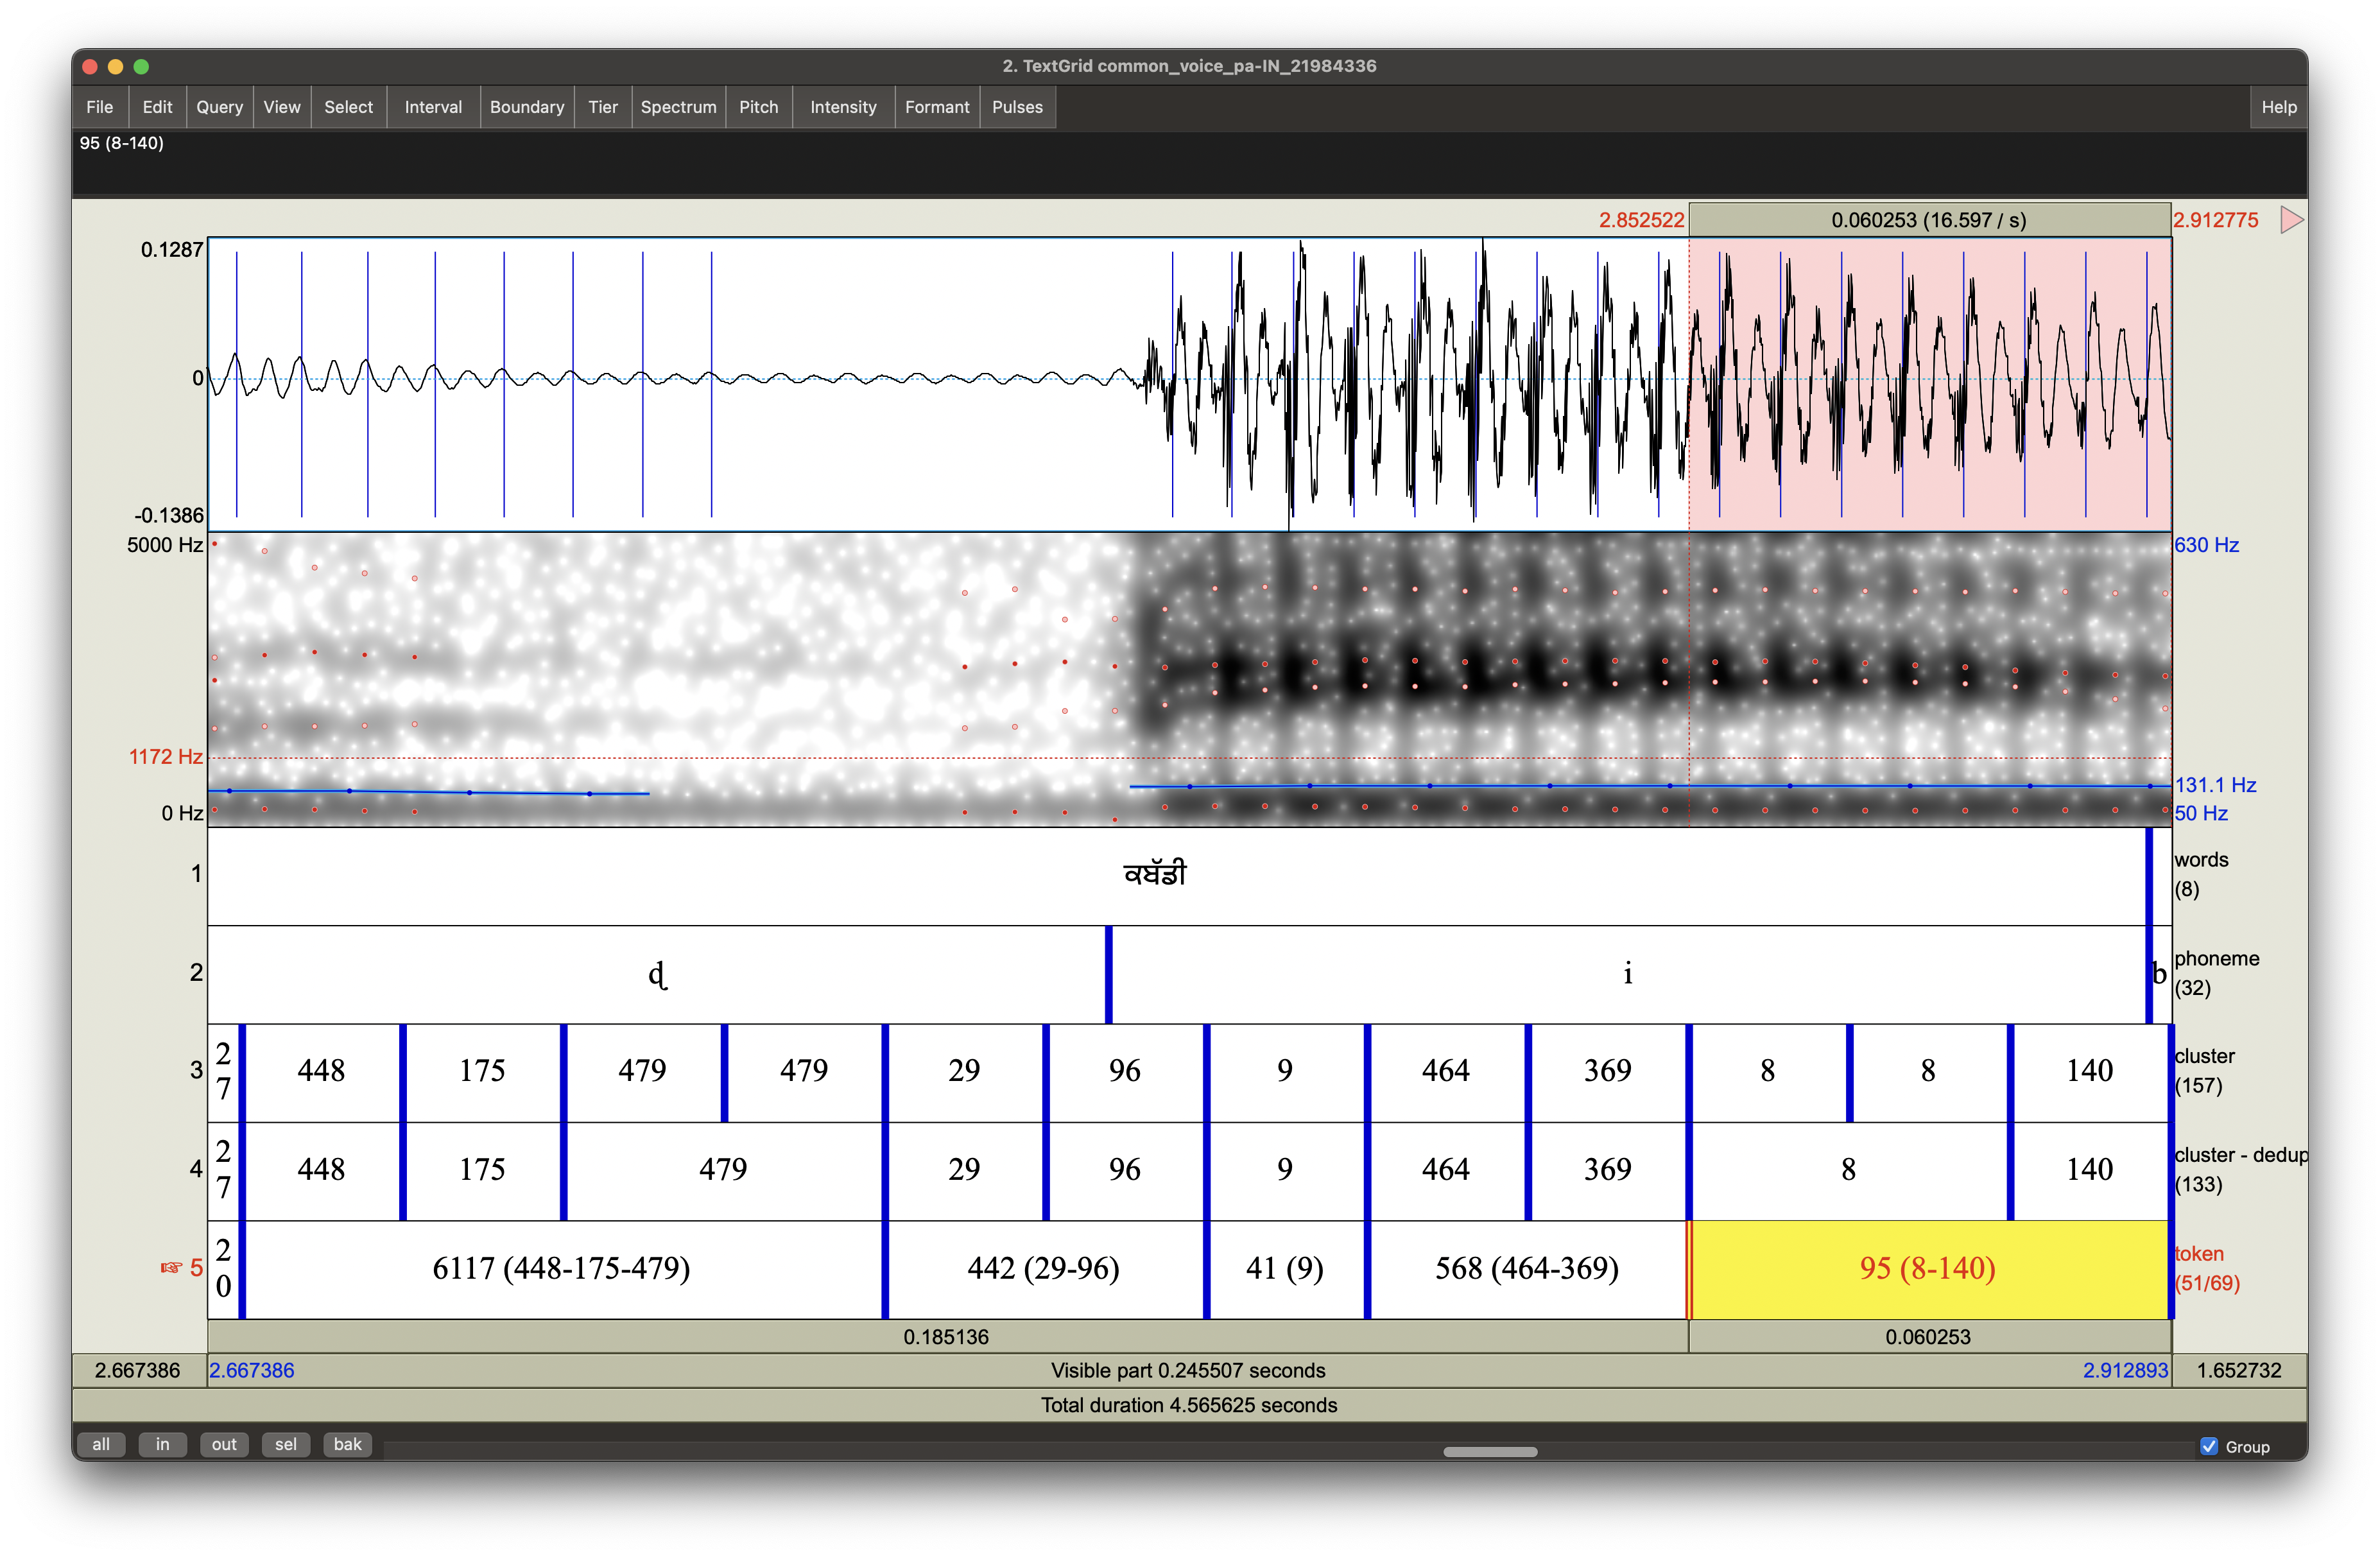
\includegraphics[width=0.975\linewidth]{figures/token-phoneme-TextGrid.png}
\caption[Punjabi utterance enriched with pseudo-tokens for analysis]{\corr{Punjabi utterance enriched with pseudo-tokens for analysis.~The first two tiers (words, phoneme) are force-aligned annotations sourced from VoxCommunis \parencite{ahn-chodroff-2022-voxcommunis}.~The third tier (cluster - 49hz) consists of cluster numbers (0-499) derived by using k-means clustering to group individual time windows based on wav2vec 2.0 embeddings, and the fourth tier (cluster - dedup) retains only uniquely consecutive clusters.~The fifth tier (token) further groups unique clusters from the fourth tier based on their frequencies of co-occurrence (e.g.~the 95th most frequently occurring span, i.e. token 95, is composed to the speech sounds in cluster 8 and cluster 140).}}
\label{fig:textgrid}
\end{figure}

\end{landscape}

\corr{\noindent{}annotations from the VoxCommunis corpus as well as induced pseudo-tokens.~The first tier consists of the Punjabi word and second tier its phonemic representation /{\fontspec{LinLibertine.ttf}ɖi}/ derived via an automatic grapheme-to-phoneme conversion process.~The third tier (cluster - 49 Hz) comprises of cluster numbers derived by using a k-means model to group together each time window of speech based on their acoustic features, represented using wav2vec 2.0 embeddings extracted from the 12th transformer layer.~Given the 49 Hz emission frequency, we can observe that these evenly-spaced units are sub-phonemic and yield repetitions (e.g. `8 8 140' as appears on the right edge of the `cluster - 49hz' tier).}

\corr{~The task of tokenisation, then, is to derive coarser-grained units, i.e. temporally speaking more phone(me)-like.~First, the `cluster - dedup' tier simply deduplicates repetitions, e.g. `8 8 140' $\rightarrow$ `8 140'.~Then, based on their frequencies of co-occurrence in Punjabi, we further group these clusters into coarser-grained groups, which we term `tokens'.~As indicated on the `token' tier in Figure \ref{fig:textgrid}, sequence 8 and 140 was grouped into a single token 95, based on their frequency of co-occurrence in Punjabi.~For each token interval, we tallied for analysis the phoneme label present on the phoneme tier at the token midpoint --- e.g. the label /i/ for last `95 (8-140)' interval on the token tier in Figure \ref{fig:textgrid}.~Using the models trained on Punjabi, we then repeated the token induction process on the Hindi speech corpus and tallied the correspondences between the tokens and Hindi phoneme labels.}

\corr{\noindent{}\textbf{\textit{Results}}.~Table \ref{tab:pa-hi-tok2phon} summarises the top three phoneme labels from Punjabi and Hindi speech corpora associated with induced tokens shown in Figure \ref{fig:textgrid}.~The results show that tokens were broadly associated with a specific speech sound or a set of speech sounds.~For example, in Punjabi all occurrences of token 6117 was associated with the retroflex stop /{\fontspec{LinLibertine.ttf}ɖ}/ and similarly for token 568 with the high front vowel /i/.~These associations were also broadly similar when the tokens were induced on a Hindi corpus and compared to Hindi labels.~For example, token 41 is associated with roughly the same set of front vowels in both languages.}

\begin{table}[!h]
\centering
\renewcommand{\arraystretch}{1.55}
\begin{tabular}{@{}cll@{}}
\toprule
\multirow{2}{*}{Induced Punjabi token ID} & \multicolumn{2}{l}{Top 3 phoneme labels (\% occurrence)}   \\ \cmidrule(l){2-3} 
                                       & Punjabi corpus              & Hindi corpus                 \\ \midrule
6117                                   & {\fontspec{LinLibertine.ttf}ɖ} (100\%)                   & d (100\%)                    \\
442                                    & {\fontspec{LinLibertine.ttf}ɖ} (78\%), i (8\%), ʈ (5\%)  & i (17\%), {\fontspec{LinLibertine.ttf}ə} (17\%), e (13\%) \\
41                                     & i (50\%), e (33\%), {\fontspec{LinLibertine.ttf}ɪ} (7\%) & i (54\%), e (33\%), j (4\%)  \\
568                                    & i (100\%)                   & i (72\%), j (15\%), e (11\%) \\
95                                     & i (90\%), {\fontspec{LinLibertine.ttf}ĩ} (5\%), e (2\%) & i (55\%), m (7\%), n (7\%)   \\ \bottomrule
\end{tabular}
\caption[Correspondences between phoneme labels and pseudo-tokens induced on Punjabi and Hindi speech]{\corr{Correspondences of tokens induced on Punjabi and Hindi speech based on frequently occurring sound sequences in Punjabi corpus.~Percentages indicate proportion of phoneme label observed at mid-point of induced token interval.~Phoneme labels were obtained from grapheme-to-phoneme conversion of language text and time boundaries via forced alignment, available from the VoxCommunis corpus \parencite{ahn-chodroff-2022-voxcommunis}.}}
\label{tab:pa-hi-tok2phon}
\end{table}

\newpage

\corr{There is of course a certain degree of noise in these comparisons, given that all annotations discussed above are machine-derived --- from the phoneme labels derived via grapheme-to-phoneme conversion, to time boundaries aligned to speech via forced alignment, to the induced tokens derived based on grouping frequently occurring spans of speech.~Thus, there are bound to be certain inconsistencies.~For example, while token 442 is commonly associated with /{\fontspec{LinLibertine.ttf}ɖ}/, it is almost uniformly split across various vowels in Hindi.~Note, however, the occurrence of token 442 Figure \ref{fig:textgrid} places it at the boundary between the retroflex and vowel, and such misalignments between automatically-induced tokens and forced-aligned time boundaries may help explain this difference.~At the same time, despite such inconsistencies, we are able to observe some broad level of within- and cross-language consistency between tokens and regularly occurring speech sounds in corpora.~Given this broad consistency, these tokens may still be useful for measuring how similarly distributed speech sounds are between two corpora.}

\subsection{Comparison of similarity measures}

\textbf{\textit{Method}}. In our first analysis, we examined how well ATDS can account for the results of the Indic language experiments and how ATDS compares to other measures.~Accordingly, for ATDS, we trained the relevant wav2seq models on Punjabi (the target language), induced tokens on Punjabi and all donor languages, then calculated the token frequency vectors and computed the pairwise cosine similarities.~As in \textcite{9688276}, \corr{we also independently computed for the Indic languages} similarities using lang2vec and corpus-level means of utterance-level embeddings extracted using a pre-trained spoken language identification model \parencite[SpeechBrain:][]{ravanelli2021speechbrain}.

\noindent{}\textbf{\textit{Results}}. This analysis revealed that the two bottom-up acoustic measures provide overall a finer-grained ranking than top-down lang2vec measures.~For example, as shown in Table \ref{tab:atds_results} Feat. (a combination of all lang2vec data sources), the featural similarity, splits the four languages into two groups:~similar~(0.6:~Hindi--Marathi) and dissimilar (0.5:~Bengali--Tamil).~Additionally, we also found erroneous, perfect similarity values (1.0), resulting from identical language vectors for the category (e.g.~Phon.: Marathi-Punjabi), likely an artefact of data imputation.~These results demonstrate that while top-down data may be suitable for more noise-tolerant applications (e.g. large-scale typological comparisons), they may not be well suited for helping select donors for a specific under-described target language if the relevant metadata is unavailable or inaccurate.

While both acoustic measures accurately select Hindi as the most suitable donor, ATDS provides a better ranking of the donor languages.~As shown in Table \ref{tab:atds_results} (SB), the measure based on SpeechBrain embeddings ranks Gujarati as being as dissimilar to Punjabi as Bengali/Malayalam.~We make a similar observation as above that using embeddings from a different pre-trained model than the one to be adapted via CPT risks adding unwanted noise to an inherently hard task.~Leveraging the representations of the pre-trained model to be adapted reduces this risk, reflected in ASR improvement being most correlated with ATDS (\textit{r}~=~0.89; \corr{note that similarity is positively correlated with word error rate reduction, WERR}).

\begin{figure}[!ht]

\vspace{2em}

\centering
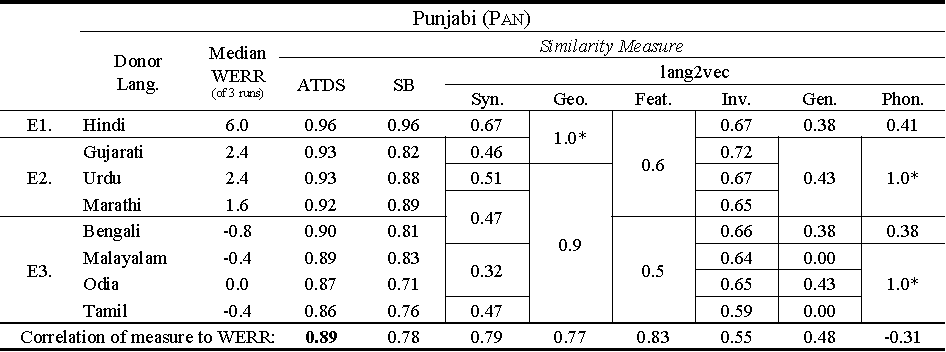
\includegraphics[width=1\textwidth]{figures/sigtyp2024-atds-l2v-sb}

\captionof{table}[Acoustic Token Distribution Similarity (ATDS) measure between Punjabi and donor language predicts downstream speech recognition performance as measured by word error rate reduction (WERR)]{Acoustic Token Distribution Similarity (ATDS) measure between Punjabi and donor language predicts downstream speech recognition performance as measured by word error rate reduction (WERR; higher is better) when fine-tuning the wav2vec 2.0 XLSR-128 model adapted using continued pre-training (CPT) on 10 hours of target and 60 hours of donor language speech.~Other similarity measures for comparison are derived embeddings of the SpeechBrain language identification model and from the lang2vec database (syntactic, geographic, featural, inventory, genetic, and phonological).~* indicate erroneous similarity scores resulting from identical, imputed vectors within the database.~Correlations (Pearson's \textit{r}) calculated using 24 data points (8 donor languages x 3 CPT runs per language with different donor data in each run).}
\label{tab:atds_results}

\vspace{3em}

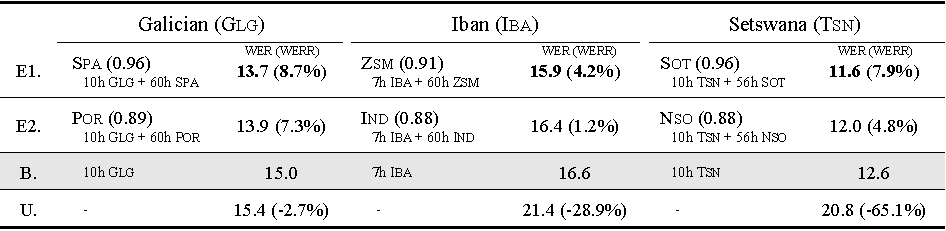
\includegraphics[width=1\textwidth]{figures/sigtyp2024-galician-iban-setswana.pdf}

\captionof{table}[Acoustic Token Distribution Similarity (ATDS) validated on three other target languages (Galician, Iban, Setswana)]{Validation of the Acoustic Token Distribution Similarity (ATDS) measure for predicting target language automatic speech recognition (ASR) performance as a result of continued pre-training (CPT) of the wav2vec 2.0 XLSR-128 model using mix target and donor language data.~For each target language (Galician, Iban, Setswana), U. indicates ASR performance from using the unadapted XLSR-128 model, B. indicates performance from CPT adaptation with only target language data (7--10 hours), and E1--E2 using target language data supplemented with 56--60 hours of donor language data.~Parentheses next to donor language names indicate ATDS to the target language.~Percentages within parentheses indicate word error rate reduction (WERR; higher is better), relative the baseline word error rate (B) within the same column.~Donor language codes are: Spanish (S{\footnotesize{}PA}), Portuguese (P{\footnotesize{}OR}), Malay (Z{\footnotesize{}SM}), Indonesian (I{\footnotesize{}ND}), Sesotho (S{\footnotesize{}OT}), Sepedi (N{\footnotesize{}SO}).}
\label{tab:valid_results2}

\end{figure}

% \begin{figure}[!ht]
% \centering
% 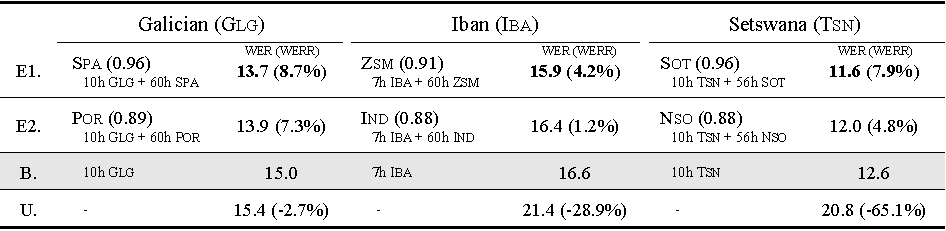
\includegraphics[width=1\textwidth]{figures/sigtyp2024-galician-iban-setswana.pdf}

% \captionof{table}{Validation of the Acoustic Token Distribution Similarity (ATDS) measure for predicting target language automatic speech recognition (ASR) performance as a result of continued pre-training (CPT) of the wav2vec 2.0 XLSR-128 model using mix target and donor language data.~For each target language (Galician, Iban, Setswana), U. indicates ASR performance from using the unadapted XLSR-128 model, B. indicates performance from CPT adaptation with only target language data (7--10 hours), and E1--E2 using target language data supplemented with 56--60 hours of donor language data.~Parentheses next to donor language names indicate ATDS to the target language.~Percentages within parentheses indicate word error rate reduction (WERR; higher is better), relative the baseline word error rate (B) within the same column.~Donor language codes are: Spanish (S{\footnotesize{}PA}), Portuguese (P{\footnotesize{}OR}), Malay (Z{\footnotesize{}SM}), Indonesian (I{\footnotesize{}ND}), Sesotho (S{\footnotesize{}OT}), Sepedi (N{\footnotesize{}SO}).}
% \label{tab:valid_results2}

% \end{figure}

\subsection{Validation of ATDS beyond Indic languages}

\textbf{\textit{Method}}.~In our second analysis, we examined whether the ATDS measure generalised beyond the Indic languages through identical CPT experiments on a typologically varied set of target languages.~We selected triplets of languages consisting of 1) a target language,~2) a language more similar to the target as measured by ATDS,~and 3) another language relatively farther.~As summarised in Table \ref{tab:valid_results2}, the target languages were Galician (West-Iberian), Iban (Malayic), and Setswana (Sotho–Tswana).~For Galician, ATDS predicted that Spanish (S{\footnotesize{}PA}: 0.96) was more similar than Portuguese (P{\footnotesize{}OR}: 0.89); for Iban, Malay (Z{\footnotesize{}SM}: 0.91) more than Indonesian (I{\footnotesize{}ND}: 0.88); and for Setswana, Sesotho (S{\footnotesize{}OT}: 0.96) more than Sepedi (N{\footnotesize{}SO}: 0.88).

\noindent{}\textbf{\textit{Results}}.~These CPT experiments are summarised in Table \ref{tab:valid_results2}.~We first note the large difference between Galician and the other languages in the improvement yielded by CPT baselines (B) compared to fine-tuning the unadapted XLSR-128 (U).~As we sourced Galician data from CommonVoice (on which XLSR-128 was already pre-trained), CPT yields little further gain (U. 15.4\% vs. B. 15.0\%).~By contrast, ASR performance was much improved via CPT adaptation for both Iban (U. 21.4\% vs. B. 16.6\%) and Setswana (U. 20.8\% vs. B. 12.6\%).~These results constitute further evidence that directly fine-tuning massively multilingual models can yield sub-optimal performance for under-represented languages and that continued pre-training can help close this performance gap.

We found that the ATDS predictions are borne out for all three target languages (even for Galician in spite of relatively reduced benefits).~As shown in Table \ref{tab:valid_results2} for each of the target language columns (Galician, Iban, Setswana), larger improvements in target language ASR performance are observed as a result of continued pre-training on target language data supplemented with data from a more similar language as measured by ATDS than a less similar one (respectively, rows E1.~vs.~E2).~Combined with results for Punjabi above, our findings altogether provide strong evidence for the effectiveness of ATDS for predicting positive transfer between target and donor languages for CPT-based model adaptation.

\section{Conclusion}
\label{sec:sigtyp:conc}

For developing automatic speech recognition (ASR) systems for languages with very few resources, I demonstrated that massively multilingual pre-trained models for speech can be successfully adapted via continued pre-training using a mix of data from the target language and supplemental data from a similar, higher-resource `donor' language.~Additionally, I motivated and proposed the Acoustic Token Distribution Similarity (ATDS) --- a novel measure of similarity to predict positive transfer between a donor and target language.~Across a set of typologically different target languages (Punjabi, Galician, Iban, Setswana), I showed that the ATDS between the target language and its candidate donors precisely predicts target language ASR performance.

This predictive capability of ATDS can be attributed to leveraging the knowledge of the pre-trained model to be adapted, its inductive biases and training objectives, and the distributions within the candidate datasets that will be used to adapt it.~It is indeed expected that this measure then is able to predict downstream task improvements better than measures based on other models or external information --- the latter of which is not always available or reliable for under-described languages.~Given the high cost associated with continued pre-training, however, I argue that using a well-calibrated, task-specific measure minimises the chance of costly, unexpected outcomes.

These findings, naturally, come with some limitations.~To focus on exploring transfer between languages, the standard wav2vec 2.0 pre-training recipe was used.~I acknowledge that this requires a large compute budget beyond what is affordable in many low resource scenarios.~In future, I hope to investigate whether or to what extent transfer learning can be combined with more compute-efficient adaptation methods.~To conduct a systematic study of pairwise transfer, I used domain-matched, high-quality ASR datasets containing mostly read speech and only examined sourcing data from a single donor language.~Questions relating to multi-donor and multi-domain transfer, how such interactions affect downstream performance in the target language, as well as experiments with real-world documentation data will need to be addressed in future research. 

I make a final observation here that various target-donor language pairs where successful transfer was observed exist in linguistic situations with significant, sustained contact.~For example, Galician is a minoritised language in Spain and virtually all Galician speakers are bilingual in Spanish \parencite{de2020phonetic}.~Similarly, \textcite{macaire-etal-2022-automatic} report that fine-tuning a model pre-trained on French was particularly successful for Gwadloupéyen and Morisien, two French-based creole languages.~These findings suggest that to develop truly inclusive speech technologies in a resource efficient manner, what will be required is a nuanced understanding of what factors linguistic and non-linguistic yield sufficiently high levels of cross-lingual similarity which in turn permit positive transfer.

\end{document}

